\subsubsection*{Training Insights}
ResNet152V2 was amongst the most successful of all models trained. It achieved a standard deviation of $ \sigma \le 1.8$ on five occasions. As seen in the best performing model (see \autoref{fig:resnet152v2_best_history}), many trainings began with only modest progress but after a few thousand epochs the training was able to make huge improvements and training loss decreased rapidly. This also allowed the validation loss to settle after repeated outbursts. The ability to find useful features after long training and to be able to continue training without overfitting is one of the key advantages I witnessed during training.   
\subsubsection*{Best Performing Model}
ResNet152V2 was able to make the best predictions out of all nine trained models. With a $\sigma$ of $1.34$ it was only marginally worse than the basic CNN with a standard deviation of $\sigma \sim 1.30$. As brought up before, ResNet152V2 training was able to make rapid improvements after around 1800 epochs and both training and validation loss was able to improve because of that. Moreover, there is no visible overfitting going on which is indicated by the steady validation loss and the training predictions (see \autoref{fig:best_perf_resnet152v2_b}).

\begin{figure}[H]
\centering
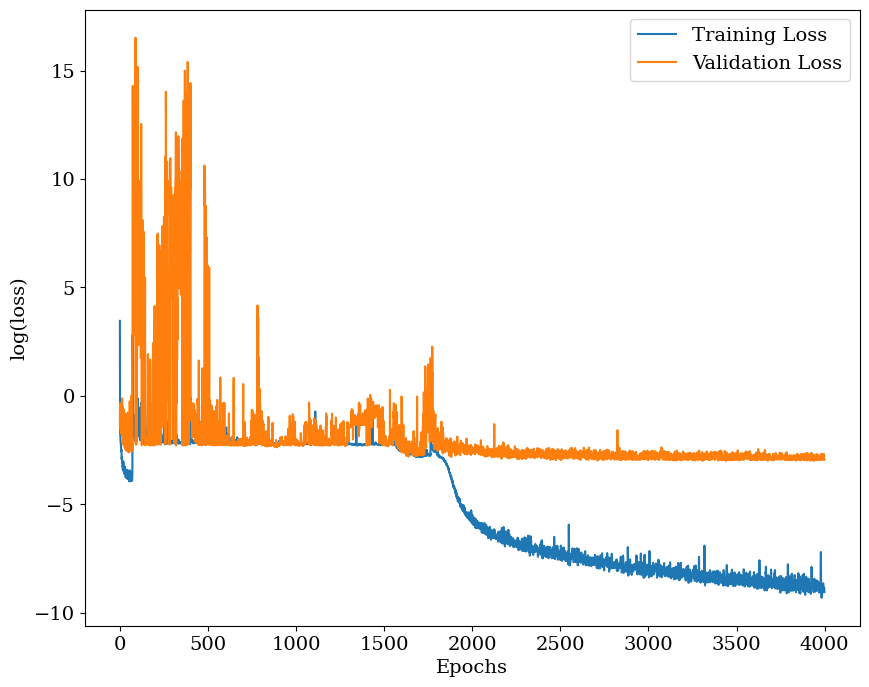
\includegraphics[width=.667\textwidth]{images/Chapter4/Res152V2/res152v2_history.png}
\caption{Training history of the best performing ResNet152V2 model.} 
\label{fig:resnet152v2_best_history}
\end{figure}

As seen with other ResNet models, this model also overestimated smaller galaxy clusters and underestimates the masses of bigger galaxy clusters with an overall trend on underestimating ($\mu = 0.055$). Especially in a mass range between $\log{(M_{500}^{\text{true}}/M_{\odot})} = 14$ and $\log{(M_{500}^{\text{true}}/M_{\odot})} = 14.5$ the predictions seem to be even better which could mean that it is easier for the model to estimate the masses of larger galaxy clusters.

\begin{figure}[H]
\centering
\begin{subfigure}{.46\textwidth}
  \centering
  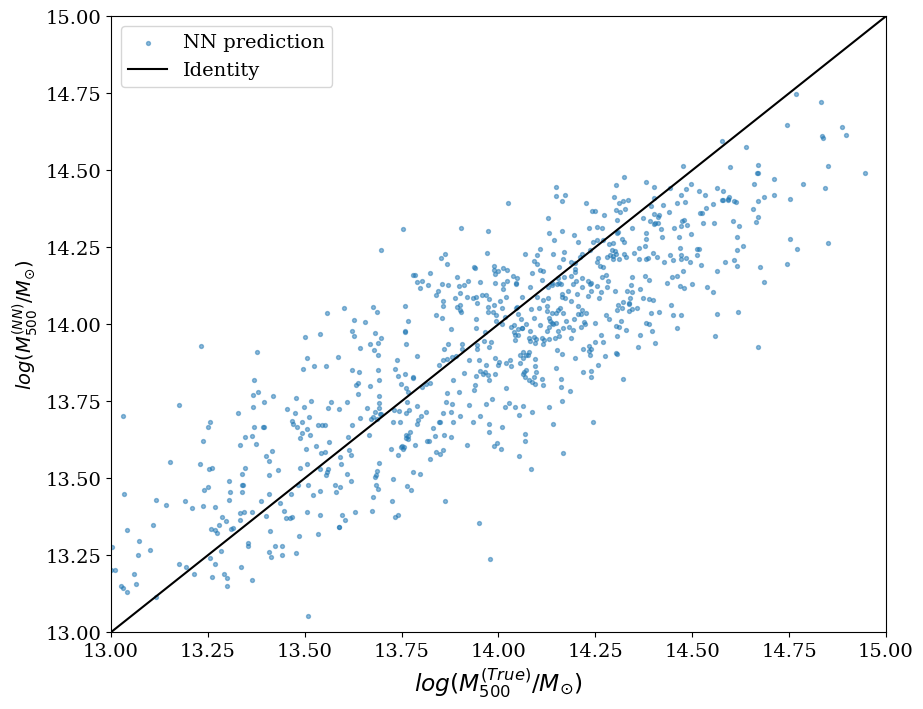
\includegraphics[width=\linewidth]{images/Chapter4/Res152V2/res152v2_test.png}
  \caption{Model predictions on the test set.}
  \label{fig:best_perf_resnet152v2_a}
\end{subfigure}%
\hspace{.6em}
\begin{subfigure}{.46\textwidth}
  \centering
  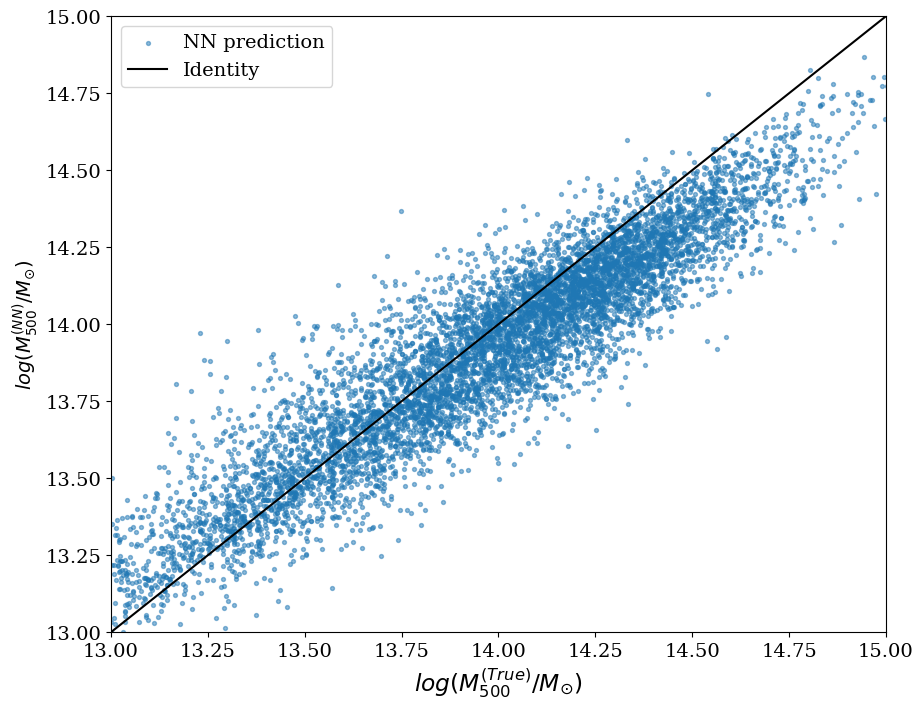
\includegraphics[width=\linewidth]{images/Chapter4/Res152V2/res152v2_train.png}
  \caption{Model predictions on the training set.}
  \label{fig:best_perf_resnet152v2_b}
\end{subfigure}
\begin{subfigure}{.46\textwidth}
  \centering
  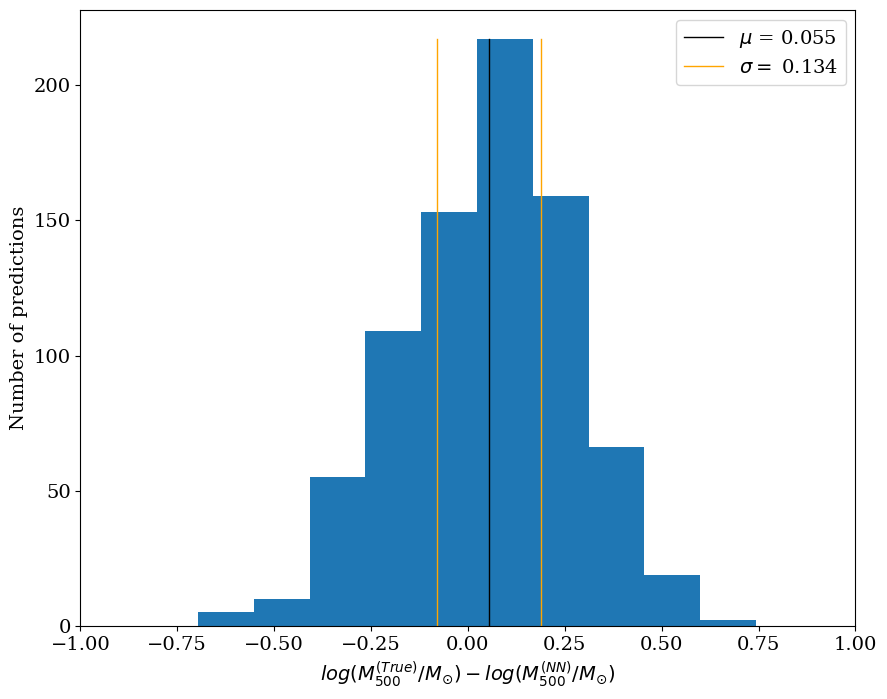
\includegraphics[width=\linewidth]{images/Chapter4/Res152V2/res152v2_test_hist.png}
  \caption{Histogram of model predictions on the test set.}
  \label{fig:best_perf_resnet152v2_c}
\end{subfigure}%
\hspace{.6em}
\begin{subfigure}{.46\textwidth}
  \centering
  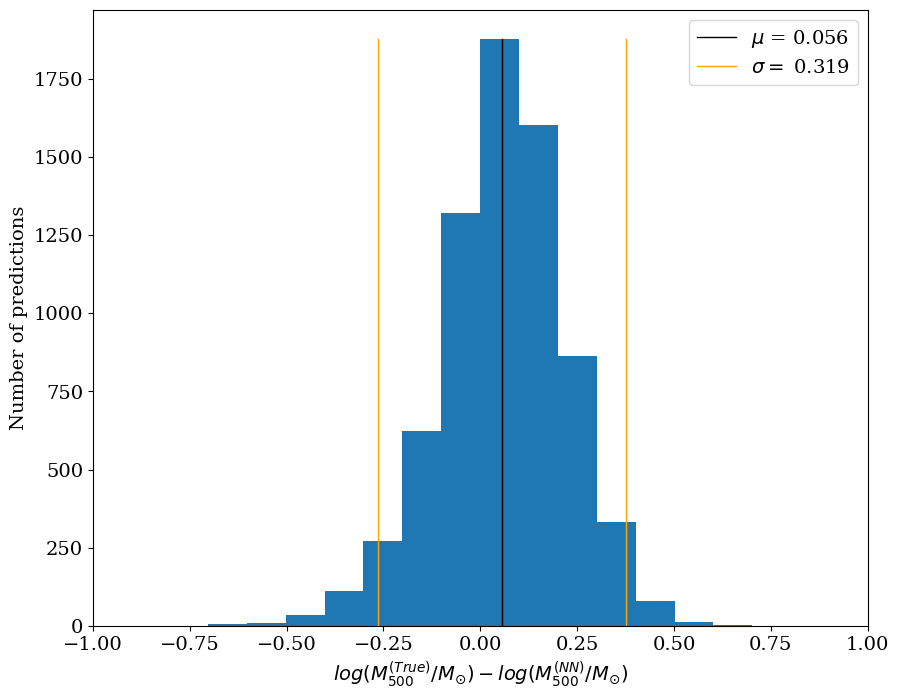
\includegraphics[width=\linewidth]{images/Chapter4/Res152V2/res152v2_train_hist.png}
  \caption{Histogram of model predictions on the training set.}
  \label{fig:best_perf_resnet152v2_d}
\end{subfigure}
\caption{Results of the best overall performing deep network. $\sigma$ is quite high at the training set as a result of a few very bad predictions outside of the mass range. } 
\label{fig:best_perf_resnet152v2}
\end{figure}

One thing worth noting with the training predictions is that the model put a few galaxy clusters on masses that are outside of the mass range. This results in the standard deviation of the training set being way higher ($\sigma = 0.319$) than the standard deviation of the test set. This makes it a bit harder to spot overfitting but considering the prediction's spread in \autoref{fig:best_perf_resnet152v2_b} the model is most likely not overfitting. Finding improvements to this model might not be so easy but as with the other deep models a smaller learning rate could help to improve prediction accuracy.